\documentclass{standalone}
\usepackage{tikz}
\usepackage{graphicx}

\begin{document}
    \begin{tikzpicture}

        % Define coordinates for images
        \node (img0) at (0,0) {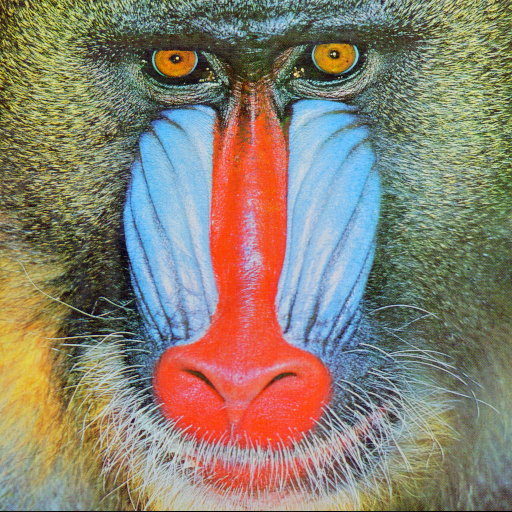
\includegraphics[width=2cm]{images/forward-process-0.png}};
        \node (img1) at (3,0) {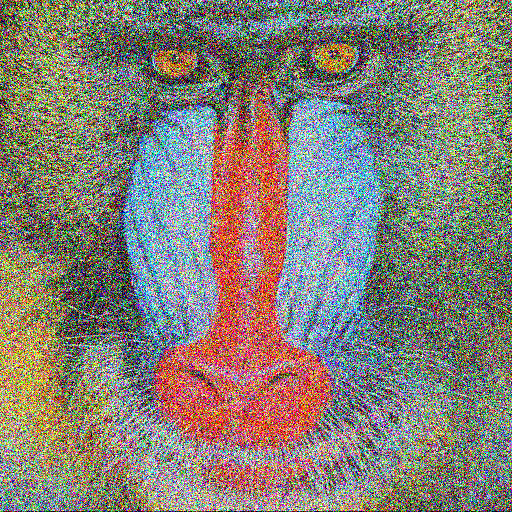
\includegraphics[width=2cm]{images/forward-process-5.png}};
        \node (img2) at (6,0) {
\includegraphics[width=2cm]{images/forward-process-10.png}};
        \node (img3) at (9,0) {
\includegraphics[width=2cm]{images/forward-process-15.png}};
        \node (img4) at (12,0) {
\includegraphics[width=2cm]{images/forward-process-20.png}};

        % Add labels below the first and last images
        \node[below=1cm] at (img0) {$x_0$};
        \node[below=1cm] at (img4) {$x_T$};

        % Draw arrows from the center-right of each image to the center-left of the next
        \draw[->, thick, color=red!70] (img0.east) -- (img1.west);
        \draw[->, thick, color=red!70] (img1.east) -- (img2.west);
        \draw[->, thick, color=red!70] (img2.east) -- (img3.west);
        \draw[->, thick, color=red!70] (img3.east) -- (img4.west);

    \end{tikzpicture}
\end{document}
